\documentclass[../main/Feedback.tex]{subfiles}
\begin{document}
\section{Introduction}
One process that is time consuming, and often one that we cannot avoid, is filling web forms with information.
These might be mundane, like registering with a new website, procedural, like online banking, or complex and important, like completing a tax return. Regardless, we encounter them frequently, if not many times a day. Complex forms, like tax returns and car insurance claims, can be very difficult for users, potentially also creating a significant amount of stress.
From a Usability perspective, the forms should be designed so they are intuitive and easy to use, aiding users through the filling process, and helping them avoid making errors. Although usability has many facets \cite{bevan2001international}, one concern is for the mental workload (MWL) of the users \cite{bevan1997methods}, which is typically measured using retrospective subjective forms \cite{nasatlx}. In this paper, however, we explore the use of concurrent objective measure of MWL: functional Near Infrared Spectroscopy (fNIRS). Although research has demonstrated that this technology is suitable for user study conditions, the evidence has been based upon constrained psychology tasks like N-Back tests \cite{ayaz2007detecting,herff2013mental,molteni2008activation}. Here, we demonstrate that fNIRS can be easily integrated into typical usability testing conditions, as we compare alternative designs for an online insurance claim form.

Mental workload is \emph{``the relationship between primary task performance and the resources demanded by the primary task''} \cite{wilson2015evaluation}. In their recent model of MWL, Sharples and Megaw highlight that both high and low MWL, can reduce performance ~\cite{wilson2015evaluation}. As a task complexity increases, performance reduces. Conversely, a repetitive task that does not utilize a person's mental or physical resources may result in boredom and apathy \cite{afergan2014dynamic}, which also means that a user becomes prone to errors \cite{pekrun2010boredom}.
%Web form filling tents to be a repetitive task which sometimes can become automatic.
%If users reach such state, they might not only dislike the process or task of form filling, but they are
It is therefore important in the field of HCI evaluation and Usability to understand users' capabilities and limitations, in order to assess the demands placed upon them.
\begin{figure} [h]
	\centering
	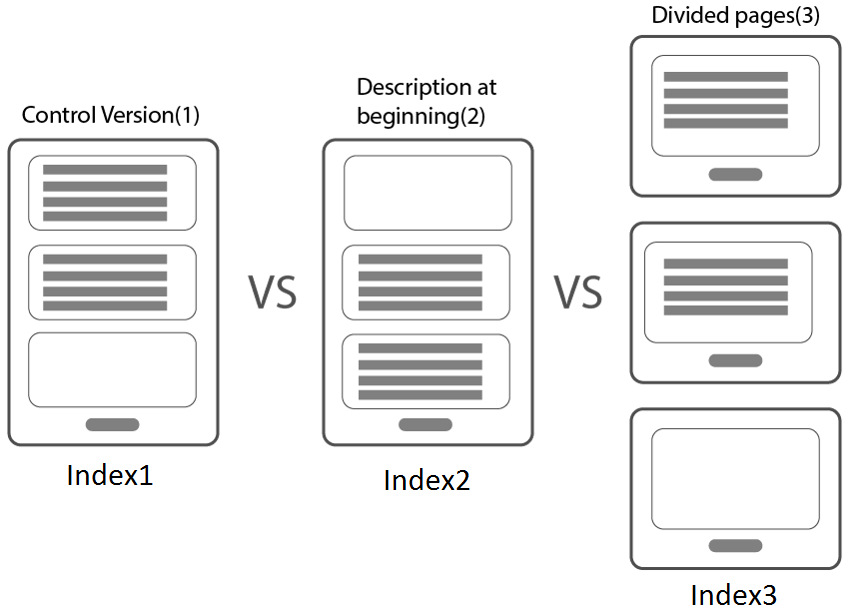
\includegraphics[width=0.8\linewidth]{../figures/layout-variations}
	\caption{A sketch of the three web form layout variations investigated.}
	\label{fig:layout-variations}
\end{figure}

The aim of this usability study is to evaluate a web form filling interface for the insurance domain, and we use the example of online auto insurance claim process.
We therefore evaluate three variations in the layout of the insurance claim form, as shown in Figure~\ref{fig:layout-variations}, and examine the effects on users preference, emotional response, workload, and performance.
The first variation (Index2) of the default web form examines whether summarizing at the beginning of an insurance claim form might make the process easier.
The second (Index3), is looking at ways to make the form easier to fill and clearer by dividing the form fields into separate, sequential subforms.
\subsection{Usability and Web Form Filling}	
Web form filling is a task often encountered within our daily activities, however, according to our knowledge, there is scarcely any \emph{empirical} research literature for this topic.
Most of the research on web form filling and design is focused in optimizing the experience and accessibility for elderly population \cite{chadwick2003web,lines2006online,sayago2007some,sayago2012selective}.
W{\"a}stlund et al \cite{Wastlund20081229} compared two web page layouts, one in which all the text is on single page, and one where the text is separated over four pages, and concluded that users experienced less workload with the divided web form.
Further research \cite{jarrett2009forms,wroblewski2008web} also suggest splitting long web forms into several pages in order to improve the process.
It is suggested that the longer it takes for a task to be completed (short or long term) the more the perceived frustration users experience \cite{bessiere2004social,mendoza2005usability}. Time to complete was also considered in our study.
%In reviewing positive and negative affect and their implications for design Norman \cite{norman2002emotion} proposes that ``Positively valenced affect broadens the thought processes hence, enhanced creativity''. Therefore, increase in task performance should be observed when a user has positively valenced affect towards certain interface. Suggesting that emotional valence plays pivotal role in task performance.

The design of web form interfaces is often based on usability guidelines, as they are widely accepted in practice.
The two most popular usability heuristics are those of Nielsen \cite{nielsen1990heuristic}, and Shneidermann \cite{shneiderman1992designing}.
%They express similar suggestions, such as maintain consistency, provide feedback, support expert users, prevent and optimize error messages, provide help documentation, permit easy reversal of information, and minimize working memory load. %Designers, however, have
%Consequently, the design of the tested variations in this study is informed by them.
Because both of them advocate minimizing the load on working memory, we consider that reducing MWL will provide better user experience. This, therefore, motivates our concern with being able to accurately measure MWL, as most measures are summative retrospective and subjective assessments provided by users after completing an entire task. With a concurrent objective measure, as proposed for fNIRS, ideally we would be able to examine the MWL at different parts of the task, and to combine with techniques like Think Aloud Protocol \cite{pike2014measuring} in usability testing.
%In addition, because usability of certain interface depends on the context, user differences, and that there is not perfect solution to a interface problem, and designers often have to make tradeoffs\cite{norman1986user}, we will rely on cognitive science in order, to predict which layout is more appropriate.


\subsection{Measuring Mental Workload}
%The concept has been explained differently by different authors.
%Sharples and Megaw \cite{wilsonChapter2015evaluation} described the effect of workload as ``the relationship between primary task performance and the resources demanded by the primary task''.
%They also discuss how user performance could be influenced by the mental workload, pointing out two causes: underload and overload.
%A number of subjective and objective methods have been proposed for evaluating users workload, including primary and secondary task analysis, subjective questionnaires and physiological techniques.

\textbf{Subjective measures} are based upon user opinions and capture the experienced users' efforts during tasks.
Due to their simplicity, cheap running costs and high validity they tend to be the most used and accepted workload measures.
One of the most used subjective technique is the multidimensional NASA-TLX scale \cite{nasatlx}.
Using the 6 sub-scales, it provides high diagnosticity, identifying different aspects of workload. Other such measures include SWAT \cite{reid1988subjective} and the Workload profile \cite{tsang1996diagnosticity}. Longo et al. \cite{longo2012importance} compared the three measures mentioned above in a web browsing/searching task, and observed correlations in the results of the three measures claiming that they measure the same concept of workload.
%One concurrent alternative is to poll users for their mental workload levels at 30s intervals during a task, using an Instantaneous Subjective Assessment (ISA) \cite{brennan1992experimental}, however many have observed the interruption that this creates and that it often increases mental workload during tasks.

%
%Between the uni-dimensional scales, Cooper-Harper \cite{cooper1969use} is one of the most popular among ergonomists.
%It was originally designed for the aircraft domain, however a modified cooper-Harper scale\cite{wierwille1983validated} was created for application in all other fields.
%As workload is influenced by different environmental and personal factors \cite{rouse1993modeling}, the concept of workload should be considered as multidimensional concept, in order to improve diagnosticity.
%NASA-TLX \cite{nasatlx}, SWAT \cite{reid1988subjective} and Workload profile \cite{tsang1996diagnosticity} are widely used multidimensional workload scales.
%NASA-TLX is based on rigorous laboratory research, and it is relatively easy to administer.
%In addition, a single measure of workload can be weighted, although it is not necessarily required because there is high correlation between weighted and unweighed results \cite{byers1988workload}.
%The SWAT subjective scale is also widely used, however the process of implementation is laborious and more complex than the other subjective scales.
%The other popular scale is Workload profile(WP) \cite{tsang1996diagnosticity} scale which is basen on the Wickens multiple resources model, and asks questions about each of the four dimensions proposed by the theory.
%Hence, it is very useful in dual task experiments. Finally, Longo et al. \cite{longo2012importance} compared the three measures mentioned above in a web browsing/searching task, and observed correlations in the results of the three measures claiming that they measure the same concept of mental workload.


\textbf{Psychophysical measures} are used to give objective data about MWL by not relying on subjective scales or performance measures.
They can be obtained by recording variable heart rate \cite{backs1994metabolic}, electrodermal response (EDR) and galvanic skin response (GSR) \cite{collet2014measuring,shi2007galvanic}, pupil dealation  \cite{beatty1982task}, imaging the brain \cite{balconi2015hemodynamic}, and facial skin temperature \cite{stemberger2010thermal}.
These techniques detect the change in the arousal from the autonomic nervous system level which can be inferred to as MWL.
However, different psychophysical measures capture different aspects workload \cite{cain2007review}, therefore consideration should be put in choosing the most appropriate measure for the given task.

Recent research has shown that fNIRS is a suitable brain measurement technique for HCI studies \cite{maior2015examining,pike2014measuring,solovey2009using} as it provides useful information about the user while allowing for more normal interaction with a computer system.
fNIRS uses blood oxygenation, rather than electrical levels that are affected by limb movement, for determining the activation of areas in the brain, where more blood flow indicates higher activity.
This makes it non-invasive, portable, and suitable for periods of extended monitoring relative to other neuroimaging techniques.
fNIRS measures the delivery of blood to active neuronal tissues and it is designed to be placed directly upon a participant's scalp, typically targeting the prefrontal cortex (PFC).
It has been suggested by cognitive neuroscience studies that PFC is involved in higher order cognition \cite{braver1997parametric} and emotion processing \cite{damasio1996somatic}. In 2009, using abstract psychology tasks, Hirshfield et al \cite{hirshfield2009brain} concluded that fNIRs should be suitable for evaluating usability. Later, Peck et al \cite{peck2013using} used hemodynamic data from fNIRS to compare and evaluate different data representations using memory tasks.
Peck et al found a negative correlation between the fNIRS levels of Hbr data and NASA-TLX, which was further confirmed by Maior et al \cite{maior2014continuous}.

In this paper, we examine the prospect of using fNIRS to measure MWL within a typical usability study. Although the work above has looked at using fNIRS in HCI user studies, it has all focused on proving its value using psychology experiments. Our primary contribution is to demonstrate how MWL can be objectively measured during usability testing to evaluate user interfaces for form filling. Further, as a secondary contribution, we also demonstrate that fNIRS can translate from constrained psychological tasks to more natural ones and still provide insight into MWL.
\end{document}



%Other fNIRS studies experiment with simple tasks, like mental arithmetic, and n-back tasks. Accordingly, we want to implement the fNIRS device in a user trial evaluation study of an web interface because it is often encountered task in our daily lives.




	%Uers often has to fill web pages containing more than 10 forms for example, when registering for a web site, posting classified ad, or sending online insurance claim. Sometimes this is really important in Human computer interaction(HCI) viewpoint, like filling insurance claim forms, and online banking to be intuitive and aiding the user through the process. To achieve that web forms should support the users working memory\cite{nielsen1990heuristic,shneiderman1992designing} by minimizing the effort to perceive, process and respond to the web form. That is why we are interested in measuring the mental demands imposed by the web form filling task. Furthermore, it has been suggested that attractive interfaces increase creativity\cite{norman2002emotion} of the user. Hence, it can be of high value for the researchers to know what workload and emotional state the users are experiencing during interaction with a certain interface.
	

	


	%We aim to find a way to improve web interfaces that has more than 10 forms, and are considered long forms, as this process is often encountered during daily web surfing, for example, when user registers to a new web site, or enter information for financial institutions, like insurance companies and banks. We strive to find more generalizable results that can produce certain web form design guidelines for interacting with long forms. Accordingly, we decided to test the layout of the web forms, and examine how it influences user performance. We also, aim to assess the practicality of fNIRS brain imaging technique in HCI evaluation studies.

%\subsection{Research questions}
%	In this master thesis we aim to answer the following questions:
%	\begin{enumerate}
%		\itemsep0em
%		\item Which of the three layouts elicit the least mental workload and which is more preferred by the users?
%		\item Is fNIRS sensitive method in measuring mental workload changes in web form filling task?
%		\item Can we detect emotional valence with fNIRS, from web interface that has no emotional cues.
%		\item Is fNIRS brain imaging modality practical to use in HCI evaluation studies?
%	\end{enumerate}		

% just remove comment on last page for ballancing columns.
%\balance{}


%In the HCI field  evaluation approaches ca be divided in three general categories: analytical, field study and lab study\cite{rogers2007interaction}. First, analytical methods are designed to predict user behaviour such as, heuristic evaluation or expert reviews, so no experiment has to be conducted. Second, field studies are conducted in context in order to collect relevant and valid data, like observations. Lastly, lab studies use artificial settings but the experiment variables can be controlled easier, and also, comparative tests can be conducted. Our aim of the study is to evaluate a web form filling interface for the insurance domain, and more precisely, online auto insurance claim process. Therefore we are interested in conducting lab study because we cannot simulate road accident and we are able to compare variations of insurance claim web form. Furthermore, there are variety of evaluation methods, like interviews which will give us information about what users think about the interface, or observations which will let us recognize typical behaviour of users and obstacles they encounter while using the interface.\\

%It has to be mentioned that lab studies give us the chance to prepare the environment and record more performance measures which provide valuable objective information. Typical performance measures in usability experiments are time to complete, errors encountered, and number of events. In general, mental workload and emotional valence are of high interest in HCI evaluations because measuring workload gives us important information about the task demands and also, knowing whether a user is feeling positive or negative towards an interface or task may give us valuable information about their general preferences. Furthermore, Nielsen\cite{nielsen1994measuring} suggested that user preferences correlate with user performance, thus we can rely solely on user preferences, however this is not always the case. Hence, Nielsen and Levy \cite{nielsen1994measuring} advise researchers to use combination of subjective and objective data in usability studies, in order to identify bias and provide richer information about the process. Accordingly, we have decided to employ user trials(subjective data) combined with psychophysiological measurements(objective data). In addition, functional near infrared spectroscopy (fNIRS), has been recently suggested as a promising method for HCI evaluations\cite{maior2015examining,pike2014measuring} because it was suggested to measure mental workload\cite{maior2014continuous}. Based on this, we decided to test the usefulness of fNIRS in HCI evaluation studies. \\

%Based on the information above this master thesis considers measuring mental workload and emotional valence to inform the user interface design of the insurance claim web form. The literature review will proceed in the following way: first, we will review relevant literature on web form filling and usability. Second, we discuss working memory models and the mental workload concept. Third, emotional processing literature will be revised. Fourth, current brain sensing techniques used in cognitive experiments will be reviewed and, fifht, fNIRS studies examining mental workload and emotional valence will be examined. Finally, we will summarize the reviewed literature.

%\subsection{Usability and Web form filling}	
%Web form filling is often encountered activity in daily surfing of web users, however, according to our knowledge, there is scarce of empirical research in the Human Computer Interaction(HCI) literature for this topic. First, a study by Wästlund\cite{Wastlund20081229} compared two web page layouts - one that all the text is in the same page, and one where the text is separated in four pages. Authors concluded that users experienced less workload with the divided web form(4 pages), compared to the single page web form. Second, two books specially written for web form filling design\cite{jarrett2009forms,wroblewski2008web} suggest splitting long web forms into several pages, in order to improve the process. Lastly, most of the research on web form filling and design is focused in optimizing the experience and accessibility for elderly population\cite{sayago2012selective,chadwick2003web,lines2006online,sayago2007some}.



%\subsection{Working Memory and Mental Workload}
%The concept of mental workload (MW) is intuitive in nature and it represents how busy an operator is when performing a certain task. The concept has been referred in the literature with many terms, like cognitive load, stress, strain, and arousal. Many definitions has been proposed by many authors, however researchers are still unable to find a consensus on the term[Linton et al 1989]. Wickens\cite{wickens2008multiple} defines it as ``The demand imposed by tasks on the human's limited resources, whether considered single or multiple''. Depending on the studied task at hand, knowing workload experienced by different design variations will help choose the one that generates desired operator performance. Also, in terms of operator experience of MW, Rouse et al classifies different factors like, fatigue, mood, individual differences, as person-specific workload\cite{rouse1993modeling}. Similarly, Norman and Bobrow classified operator performance on data-limited and resource-limited\cite{norman1975data}. They hypothesize that even if operator spends high amount of attentional resources, the task can have a bad representation that will degrade the performance. In contrast, resource-limited performance depends on how much attentional resources the task demands, and it can be considered that every real life task consists of combination of both.
%\subsubsection{Working memory models}
%Rather than searching for definition researchers in cognitive science use models of working memory in order to understand cognition, predict and explain workload and performance. Furthermore, theories of working memory try to define the processes going into human mind, and explain concepts such as, attention, perception, long term memory, decision making, action selection, and execution\cite{wickens-1988,baddeley1974working,miller1956magical}. 			Most of those models are based on human as information processor approach \cite{broadbent1,broadbent2,neisser,wickens-1988}, which relates the processes of human mind with those of a computer processor. Also, the framework is based on the assumption that the human operator has a limited resource capacity\cite{kahneman1973attention,wickenshollands1999} and if the task demands more resources than the capacity of the operator, workload overload is observed. Moreover, the information from the environment or the task is processed by series of processing systems, like perception, attention, short-term memory, long-term memory.			
%\begin{figure}[h]
%	\centering
%	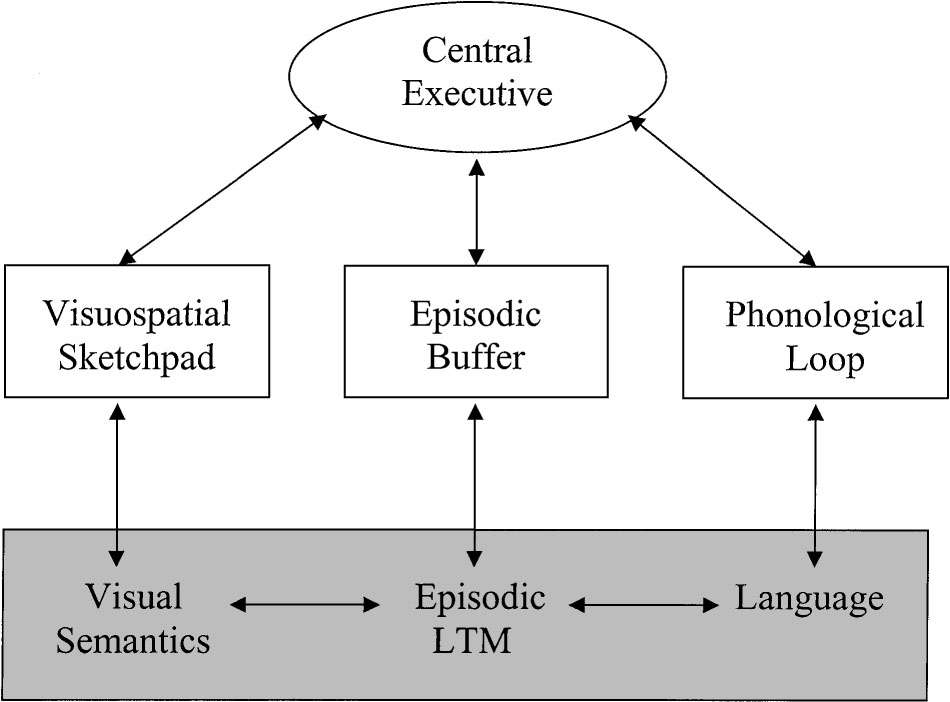
\includegraphics[width=0.7\linewidth]{baddeley-wm}
%	\caption[Baddeley and Hitch Working memory model]{Working memory model by Baddeley and Hitch, displaying the 'slave systems' visuo-spatial sketch pad, episodic buffer and phonological loop, controlled by the central executive.}
%	\label{fig:baddeley-wm}
%\end{figure}

%In attempt to describe the web form filling task we can use the working memory model from Baddeley and Hitch \cite{baddeley1974working} which processes information in verbal and spatial form. It consists of a central executive, which is acts as an administration system which controls the information input and output of its slave systems. The visuo-spatial sketch pad is involved in holding visual information in spatial form like, objects and colours. The phonological loop stores verbal information, such as words and names. And the later proposed \cite{baddeley2000episodic} episodic buffer is responsible for the storage and retrieval of memories or events. Because the task of web form filling involves multiple cognitive processes like, visual search, speech synthesis, planning, memory retrieval, decision making, thus utilizing all slave systems of the model, we can label the web form filling process as one that involves complex cognition. 		
%\begin{figure}[h]
%	\centering
%	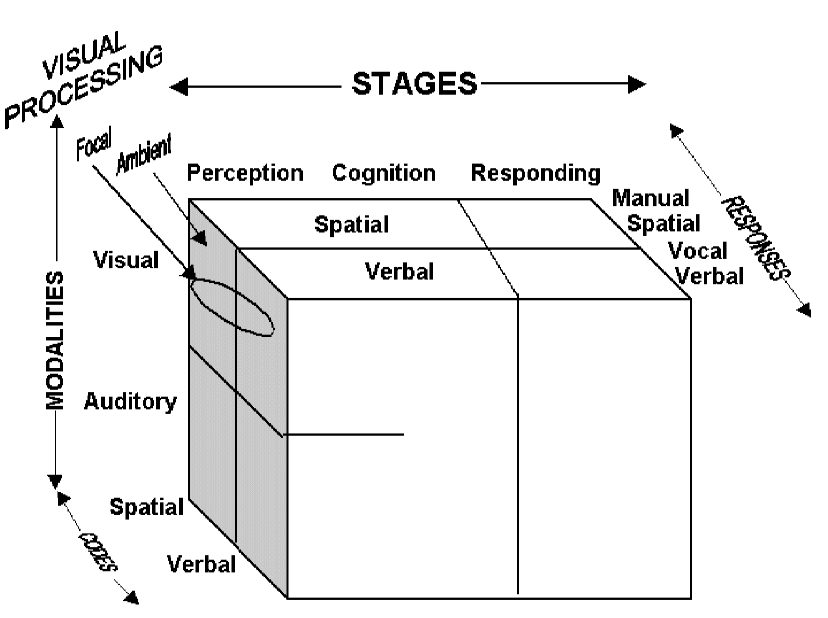
\includegraphics[width=0.8\linewidth]{mrt}
%	\caption[Multiple resource theory by Wickens]{Wickens 4-D multiple resources model consisting of two codes(spatial and verbal), 2 modalities(auditory and visual), 3 stages(perception, cognition and responding), and 2 types of responses(manual and vocal).}
%	\label{fig:mrt}
%\end{figure}

%We can also consider the multiple resources model by Wickens\cite{wickens2008multiple,wickens2002multiple} which is suited for predicting the workload of an operator performing multiple tasks at one time. The 4-D multiple resources model is visualised as 4 dimensional cube as illustrated in Figure \ref{fig:mrt}.The approach is based on four basic assumptions:

%\noindent1) in the stages of processing dimension, perceptual and cognitive tasks use different resources than response selection and execution;\\
%2) spatial activity uses different resources than verbal or linguistic activity;\\
%3) the modalities dimension, different resources are used for auditory and visual perception\\
%4) visual channels are divided on focal and ambient vision\\
%And the main argument of the theory is ``to the extent that two tasks use different levels along each of the three dimensions, time-sharing will be better'' \cite{wickens2008multiple}. The model provides an account on how different elements of the human information processor, like attention, perception, working memory, response selection and execution interact between each other. This theory is also based on research from cognitive neuroscience that suggests  different modalities have different locations in the human brain, like the auditory cortex is involved with auditory perception and the visual perception is processed mainly by the visual cortex(occupational lobe).\\

%However, mental workload can be influenced by the initial perception of the task at hand or the 'appraisal' of it. Similarly to MW appraisal is complex and multidimensional concept\cite{folkman1986dynamics,peacock1990stress} that is not well defined.


%\subsubsection{Primary and secondary task measures}
%Primary measures rely on operator performance to predict workload. However, a limitation of using primary measures alone is that an operator can spend high amount of effort but this may not be apparent from the performance\cite{wilson2015evaluation}. Consequently, primary task measures should be combined with other workload measures. An example performance measures are task completion time, number of errors, and response time. In our case we will use a combination of all but secondary task measures. Secondary task involves inclusion of a additional simple task to the primary one, which is done concurrently, if the primary task has low or moderate demand and the level of workload cannot be inferred only from the primary measure. It is used to detect when operators performance deteriorates and this is due to workload overload. However, as we are not going to use secondary measures, more explanation will provided for the other types of measurements.

%and yielded similar results, suggesting they measure the same aspects of the web task. The author infers that only one mental workload measure is required. Because mental workload is influenced by a number of factors, and therefore it is multidimensional concept, NASA-TLX is chosen as subjective measure for the experiment.


%Lavie(2005,2010) Load theory says high perceptual load decreases attention to distractions, and low perceptual load increased them. High perceptual load is experienced when, for example, driving fast a car, or playing sports. Furthermore, because it involves a lot of perceptual capacity there is no spare capacity for the attention to perceive distractions. In this case, the task has a low perceptual load because it demands only to a visual stimuli to be percieved and processed rather than with audioty, o

%\subsection{Emotion processing}
%To begin with, mood and emotion are frequently referred as separate concepts. For example, emotions are thought to last for shorter time like, several minutes, in comparison to moods which can last for a whole day or more. Also, emotions are generally caused by certain events, like winning a game, in contrast to moods where often there is no reason as to why an individual is in certain mood. However, there is no clear distinction between them because moods can cause certain emotions and emotions can cause moods. To solve that problem researchers often use the term ``affect'' to encompass both emotions and moods. Furthermore, we can define positive moods or emotions as positive affect, and negative emotion and moods as negative affect.

%There are two major approaches in describing emotions - the categorical\cite{izard2007basic} and the dimensional approach\cite{feldman1998independence}. The first one, categorises several different emotions like, happiness, sadness, anger, fear, and disgust, and often matches the subjective experience of individuals. The second one, the dimensional approach considers emotions to have two distinct dimensions of pleasure-misery (emotional valence) and arousal-sleep.
%\begin{figure}
%	\centering
%	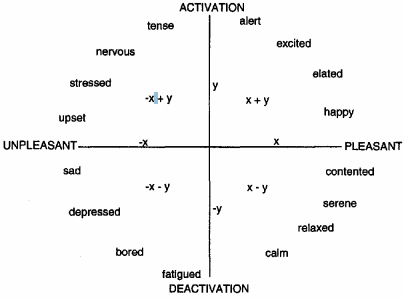
\includegraphics[width=0.7\linewidth]{two-demensional-approach-emotions}
%	\caption[Two dimensional approach of emotion]{The two dimensional approach of emotion. The x and y axes represent semantic components: x=pleasant and unpleasant emotions, and y=level of activation. The image is taken from Russell and Feldman ``Independence and bipolarity in the structure of current affect''\cite{feldman1998independence} }
%	\label{fig:two-demensional-approach-emotions}
%\end{figure}
%For example, the happy emotion can be pointed to have high positive valence and moderate activation or arousal. In contrast, the emotion of sadness has high negative valence and again moderate arousal. Furthermore, there is a considerable debate on which approach should be adopted by researchers\cite{fox2008emotion}, however we decided to use the dimensional approach because we wanted to have a numerical measure of emotional valence, which than can be compared to the objective data.

%Also, emotion processing depends on top-down(appraising a situation based on similar previous knowledge) and bottom-up(processing external stimuli) processes. The first one(top-down) is more cognitive process because it uses attention and memory in order to assign a valence to a given stimuli. The bottom up processing is influenced by external stimuli, so it uses more visual perception. Generally, there are considerable differences between them, and many theorists considers which one of them is more involved with emotion generation. However, there are many ``appraisal theories'' that suggest cognition strongly influences when we experience emotional states and what particular states we experience in a certain moment. For instance, one can appraise a non-threatening situation as threatening and therefore she will experience negative valence. Moreover, many theorists argue that appraisal is both conscious and automatic. Smith and Kirby\cite{smith2009putting} suggested two types of appraisal: one that is based on reasoning(deliberate thinking), and one that is based on activation of memories(automatic processes). The first one is claimed to be slower and more flexible.

%It has been assumed that emotional states influence cognition\cite{blanchette2010influence}, like attention, perception, decision making, and others. Also, what we remember from a situation is strongly affected by what we attended during that time\cite{eriksen1986visual}. In addition, an influential theory by Easterbrook\cite{easterbrook1959effect} suggest the number of attentional cues processed declines as arousal or anxiety increases. It can be interpreted as strong negative valence causes "tunnel vision", and positive valence produces breadth of attention. For example, a individual in highly stressful situation, like auto mobile incident, will remember only the low amount of details related to the moment of the accident. In contrast, when one is experiencing positive situation, it is likely that she will remember more unrelated details about the event. However, Harmon-Jones et al.\cite{harmon2011toward} argued that the above mentioned theory considering only emotional valence is over simplified and it lacks the addition of \textit{motivational intensity}. Generally, there are two types of motivation: approach and avoidance motivation. According to the authors the approach motivation can be low, for example listening to music, or high, for instance recognizing a attractive subject from the opposite sex. On the other hand, low avoidance motivation can be exposure to unfair situation, and high avoidance motivation can be dealing with life-threatening situation. Harmon-Jones et al.\cite{harmon2011toward} postulated that high motivational intensity leads to narrowing of the attention for both positive and negative experiences because it helps individuals to successfully accomplish tasks. On the contrary, low motivational intensity for both positive and negative experiences leads to attentional broadening because individuals leave spare attentional resources, in order to be able to encounter and react accordingly to a new and maybe more valuable situation.

%Russell\cite{russell2003core} proposed a valence model of emotion which states that significant higher activation of the left hemisphere compared to the right was associated with positive emotions, whereas significantly higher activation in the right hemisphere should be associated with negative emotion. Therefore, we can infer whether an affect was positive or negative if we measure the brain activation during an experiment.

%Generally, there are two methods that are widely used for measuring affect: objective and subjective. One subjective measurement technique is the self assessment manikin(SAM)\cite{bradley1994measuring}, which we used because it provides two scales - emotional valence and arousal. Other widely used measure is the Positive and Negative Affect Schedule(Panas)\cite{watson1988development}. However, it is more complex to use, for example, explain to participants how to use it, and also, the procedure takes more time. However, we want to avoid that because of the increasing uncomfortability of wearing fNIRS device with the time. Also, the scales had visual icons that help participants recognise what each point of the scale means. The objective techniques that try to infer emotional valence include psychophysiological measures of galvanic skin response, heart rate, respiration\cite{krumhansl1997exploratory}, and brain activity\cite{Balconi201567}. We decided to combine subjective and objective measure of emotional valence, in order to compare them and later make inferences about. We chose SAM because it is widely accepted, and easy to implement, and brain sensing technique for the objective measure, as we try to prove the left vs right hemisphere hypothesis of Davidson\cite{davidson1992emotion} which is explained below. Next, we will review brain sensing techniques and pick one suitable for this master thesis experiment.

%10. mood congruity
%11. Dual process model - fast automatic and affective system and slower effortful and more cognitive system

%\subsection{Brain sensing}
%Initially, brain sensing was used in for medical purposes, however in recent years it has been used in other fields, like cognitive psychology, and lately, for Brain-Computer interface(BCI). We review only brain sensing techniques that are suitable for measuring complex cognition and are non-invasive so it can be used in HCI experiment. First of all, the functional magnetic resonance imaging (fMRI) is measuring the haemoglobin oxygenation and deoxygenation in the brain which is referred to as blood oxygen level-dependent contrast(BOLD) signal. It uses a large magnet which causes a strong magnetic field and a short radio-frequency pulse is emitted, in order to detect areas of activation in the brain. Furthermore, MRI has high spatial resolution which detects activation in brain regions with up to 1mm precision and is suitable for distinguishing particular brain regions of activation for the studied task. Also, its temporal resolution has 2-3 seconds delay, as it takes some time for the neural activity to occur and be detected. Typical fMRI studies involve emotion induction\cite{phan2002functional,brattico2011functional} and mental arhytmetic\cite{kawashima2004functional}. However, during experiments participants should stand still and even the slightest movements can cause artefacts and distort the signal. Therefore, this technique is not suitable for HCI evaluations because subjects cannot physically move.

%Another widely used brain imaging technique is the EEG which measures electrical changes at the surface of the scalp. It is non-invasive technique, which makes it suitable for cognitive and HCI research. Waveforms with different bands are calculated from the electrical signal that can later be analysed. The strength of EEG is its temporal resolution as it can detect changes in brain activity with accuracy of a few milliseconds. However, it is highly susceptible to motion artefacts, and even the slightest movement of fingers can cause deformation of the signal. Consequently, it is not suitable for web interface evaluations because when users type on the keyboard or use the mouse will cause considerable distortions of the brain signal.

%A more recent brain imaging technique is the functional near infrared spectroscopy (fNIRS) which unlike EEG is an optical-imaging modality. Furthermore, fNIRS can detect cerebral hemodynamics by calculating the oxygenated haemoglobin(Hbo) and deoxygenated haemoglobin(Hbr). It uses infrared light which is emitted to the participants skull using emitter-detector pairs consisting of infrared LED emitter, and infrared sensors. They usually operate with two or more wavelengths (650-1000nm)\cite{scholkmann2014review}. Furthermore, because Hbo and Hbr have different light absorption coefficients and the infrared sensors can detect the reflected light from them, the concentration of Hbo and Hbr is calculated using modified Beer-Lamberts law\cite{delpy1988estimation}. The fNIRS has low temporal resolution with a 2-8 sec delay\cite{huppert2006temporal,solovey2009using} depending on the task. However, it has good spatial resolution and can detect signals 1cm inside the cortex depending on the emitter-detector configuration, and has shown good correlation with the fMRI data\cite{cui2011quantitative} for cognitive tasks.  Another advantage is that it provides a continuous data and different periods of the task can be defined and later analysed. In addition, fNIRS devices are becoming more and more portable, have high spatial resolution, and most importantly they have low sensitivity to motion artefacts which makes it particularly suitable for HCI studies\cite{maior2015examining,solovey2009using}. Hence, we decided to use fNIRS because of its applicability for usability experiments. For more comprehensive review of the fNIRS brain imaging instrumentation and methodology Scholkmann et al\cite{scholkmann2014review} article provides detailed information.
%Next, relevant studies that try to infer mental workload and emotional valence using fNIRS will be reviewed in the subsections below.
%\subsubsection{PFC, cognition and emotional processing}
%Generally, the prefrontal cortex(PFC) has been associated with higher cognitive functions by studies examining brain damaged individuals\cite{shallice1988neuropsychology,smith1997working}. Also, experiments on healthy subjects using the n-back task\cite{braver1997parametric} have supported this claim. More specifically, activation was observed in the dorsolateral prefrontal cortex (BA 9/46), inferior frontal (BA 6/44) and parietal (BA 7/44) when the task demanded more working memory resources. However, it is difficult to point which brain region is involved with which processes because one brain area is usually involved in multiple cognitive tasks\cite{brown2012common}. Moreover, Yarkoni\cite{yarkoni2011large} supported that claim by reviewing 3489 studies, which considered areas of human brain. Interestingly, activation in the same brain regions (dorsolateral prefrontal cortex, anterior insula and anterior cingulate cortex) was observed in one fifth of the studies. He used a machine learning algorithm and classified different studies into ones that assessed working memory, emotion and pain. It also, can be seen from the graphs that both working memory and emotion processing studies evoked activation in the PFC. Furthermore, individual differences in brain structure exist, especially in the PFC area\cite{thompson2001genetic}. In addition, gender differences in the brain structure are also observed\cite{cosgrove2007evolving}.

%\begin{figure}[h]
%	\centering
%	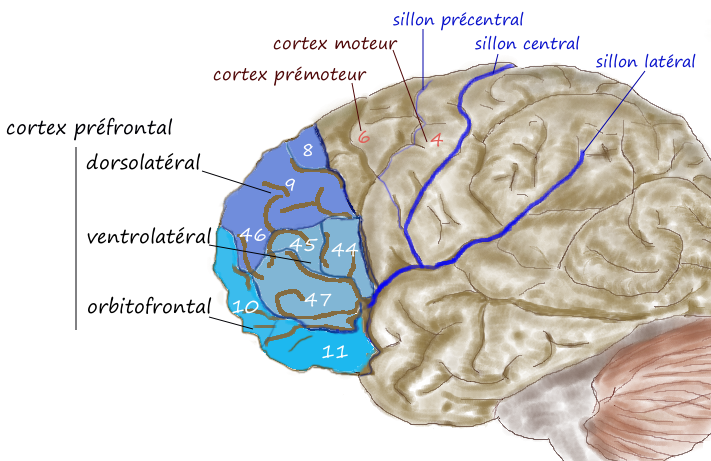
\includegraphics[width=0.7\linewidth]{../../../Desktop/Dissertation/Prefrontal1}
%	\caption[PFC brain areas]{The Prefrontal cortex functional areas. The numbers illustrated describe Broadmann areas. The picture shows the physical location of the dorsolateral cortex, the orbitofrontal cortex and the ventromedial cortex frontal cortices. fNIRS is placed between the dorsolateral and orbitofrontal cortex and measures Hbo activity with spatial resolution of 1cm.}
%	\label{fig:Prefrontal1}
%\end{figure}

%There are also evidence that the PFC is involved with emotion processing and emotion regulation\cite{davidson2002anxiety,damasio1996somatic,balconi2012detection}. More specifically, the ventromedial prefrontal cortex is suggested to be involved in the representation of positive and negative emotional states, and the dorsolateral prefrontal cortex in the representation of the goal states towards these affective states are directed. Also, it is suggested that amygdala processes threat stimuli and processes negative affect of fear\cite{davidson2002anxiety}. Furthermore, the orbitofrontal cortex in the PFC has been linked to reward processing and reinforcement learning\cite{rolls2000orbitofrontal}, therefore playing a role in the assignment in emotional valence and intrinsic motivation.

%Davidson proposed the ``valence asymmetry hypothesis''\cite{davidson1992emotion} which states that positive affect which is linked to approach motivation is experienced when the left frontal cortical region has higher activation than the right. In contrast, negative affect which is linked to avoidance motivation is experienced when more activation is observed in the right frontal cortical region compared to the left. However, the valence model of emotions by Russell\cite{russell2003core} does not connect emotional valence with approach-avoidance motivation because the emotional state of anger. Consequently, we are interested in using fNIRS in order to measure the activations in left and right frontal hemispheres and interpret the results using the \textit{valence asymmetry hypothesis}. We will review more relative studies that used fNIRS to investigate the relationship between left and right hemispheres in the ``fNIRS and Emotional Valence'' subsection below.

%\subsubsection{Fnirs and mental workload}
%In this subsection we review studies that used fNIRS in cognitive tasks. To begin with, fNIRS has been placed in different brain regions like, prefrontal cortex\cite{ayaz2012optical}, motor cortex\cite{hirth1996non} and auditory cortex\cite{plichta2011auditory}. However, because a positive correlation has been observed between the hemodynamic data from the prefrontal cortex and mental workload\cite{parasuraman2005neural} we review only studies that are measuring PFC hemodynamic activation.
%Generally, fNIRS has been used in various tasks, including remotely operating vehicles\cite{durantin2014using,ayaz2012optical}, mental arithmetic\cite{pike2014measuring}, n-back tasks\cite{durantin2014using,ayaz2012optical}, and other complex cognition tasks like video games\cite{izzetoglu2004functional,bunce2011implementation,ayaz2012optical}. However, those studies measure whether there is difference in the hemodynamics between conditions when changing the difficulty of the tasks. According to our knowledge there is only one study using fNIRS for evaluation of desktop visualisation interfaces, and more specifically comparing bar graphs and pie charts\cite{peck2013using}. They tested 16 participants, however, they could not find statistically significant difference in Hbr activation between the two graphs.
%Furthermore, it has been suggested that Hbo activation tends to be more sensitive compared to Hbr and Hbt during  mental task\cite{naseer2014online}. Another study by Plichta et al.\cite{plichta2006event} studied the reliability over time of the hemodynamic data from fNIRS and concluded that Hbo data was more reliable and stable than Hbr data. Therefore, we will use primarily Hbo for inferring mental workload and emotional valence, although Hbr and Hbt data will still be examined and results reported.


%Remotely operated vehicles \cite{durantin2014using,ayaz2012optical}
%Working memory task (n-back task\cite{durantin2014using,ayaz2012optical}, mental aritmentic\cite{pike2014measuring})
%Video game task Warship commander task\cite{izzetoglu2004functional,bunce2011implementation}
%video game air traffic controller\cite{ayaz2012optical}
%\subsubsection{fNIRS and emotional valence}
%In this section we review studies that use fNIRS data to infer about affective states measuring the hemodynamic activity of the PFC. It was not found a usability study incorporating fNIRS for measuring emotional valence. Most of the research papers use a set of predefined pictures, videos, face expressions, and words to induce positive or negative emotions.

%Most of studies use a set of affective pictures\cite{lang1997international} to elicit emotion. Balconi et al.\cite{balconi2015hemodynamic} used multiple measures from fNIRS, EEG, skin conductance, and heart rate showed affective pictures to test the valence asymmetry hypothesis. They also used the SAM subjective questionnaire to relate the psychophysiological to the self reported one. The measured Hbo from the fNIRS in the frontal right hemisphere was significantly higher when negative pictures were presented to participants. Moreover, the EEG and skin conductance data yield equivalent results. Also, it was found out that negative stimuli were more arousing according to the data from skin conductance measure. Generally, the results from this study were in accordance to the valence asymmetry hypothesis.	Another study found that positive happy face expressions were identified faster and the reaction times were lower compared to negative or angry expressions\cite{root2006left}. Also, right handers reacted faster to positive face expressions with their right hand, and to negative expressions with their left hand. The opposite pattern was observed for the left handers which reacted faster to positive stimuli with their left hand and to negative with their right hand. A similar study\cite{kong2013space} used words and facial expression to induce affect, and yield identical results as the previous one. This supports the body-specificity hypothesis\cite{casasanto2009embodiment} which states that right handers associate positive emotions with their right hand and negative emotions with their left hand. The and opposite pattern should be observed for the left handers. Consequently, it left-handers and right-handers will activate different areas of the brain viewing the same affective stimuli. Taking in consideration the limited time we have for this master thesis, and the need for significant statistical difference, we should study either right-handed or left-handed individuals.

%Furthermore, a study showing a emotional video clips\cite{leon2006differential} to participants deducted that there was a gender difference in the delay period to initial PFC activation. Later, the same authors made a similar experiment \cite{leon2007lasting} using video clips to elicit affect found out that there was activation even after finishing the video clip and the off periods should be adjusted so that post-stimuli activation do not overlap with the next condition.

%However, the above mentioned studies are designed to induce emotions, but want to study the opposite effect: can we obtain emotional valence rating from neutral web interface using fNIRS, and then infer which of the variations was objectively more preferred?

%\subsection{Summary}
%To sum up, many researchers do not consider the positive or negative affective state during task execution, and how it influences operator performance and perceived workload, we have combined multidimensional subjective workload scale (NASA-TLX) with emotional valence scale (SAM). We expect to gain better understanding of the operator performance and motivation during the web form filling task. Also, we expect to find correlations between these subjective measures and the objective measure of the mean Hbo from the fNIRS device because they are both suggested to measure mental workload and affective states.
